\section{Tutorial: PintaFotos}

En este tutorial presentaremos el componente \component{Lienzo} para
crear aplicaciones con gráficos y animaciones simples en 2 dimensiones
(2D). Construirás la aplicación \appName{PintaFotos} que permite al
usuario dibujar en la pantalla usando distintos colores, usando una
imagen de fondo y dibujando sobre ella.

\emph{Un dato histórico}: PintaFotos fue uno de los primeros programas
desarrollados para demostrar el potencial de los computadores, en la
decada de 1970. En aquel entonces, hacer algo tan simple como esta
aplicación de dibujo era algo muy complejo, y los resultados no eran
perfectos. Pero ahora, con \AppInventor, cualquiera puede rápidamente
armar una aplicación de dibujo bastante buena, lo que sirve de
excelente punto de partida para luego hacer juegos 2D.

La interfaz de usuario de \appName{PintaFotos} se muestra en
la~\Cref{fig:appUI}.

\begin{figure}[H]
\centering
% 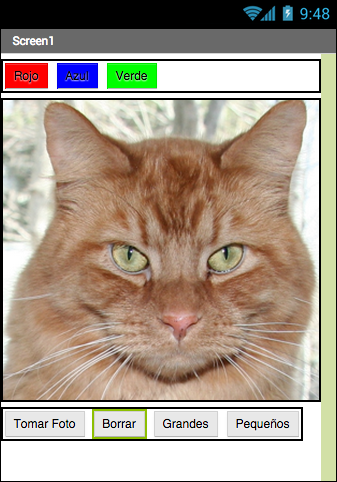
\includegraphics[scale=0.3]{PintaFotosUI}
\caption{Interfaz de usuario aplicación \appName{PintaFotos}}
\label{fig:appUI}
\end{figure}

En esta aplicación podrás:

\begin{itemize}
\item Bañar tu dedo en un tarro de pintura virtual para dibujar en
  este color.
\item Arrastrar tu dedo en la pantalla para dibujar una línea.
\item Tocar la pantalla para hacer puntos.
\item Usar el botón de abajo para limpiar la pantalla.
\item Agrandar o achicar el tamaño de los puntos con los botones
  abajo.
\item Sacar una foto con la cámara y luego dibujar encima de esta foto.
\end{itemize}

\subsection*{Qué Aprenderás}

Siguiendo este tutorial aprenderás a:

\begin{itemize}
\item Usar el componente \component{Lienzo} para dibujar.
\item Manejar las funcionalidades “touch” y “arrastrar” en la pantalla del equipo.
\item Configurar la disposición de los componentes en la pantalla.
\item Usar los controladores de eventos que reciben argumentos o
  parámetros.
\item Definir variables para recordar cosas como el tamaño de un punto
  elegido por el usuario para dibujar.
\end{itemize}

\subsection*{Para Empezar}

Aseguráte que tu computador y teléfono están configurados para usar
\AppInventor. Crea un nuevo proyecto y nombrálo \appName{PintaFotos}. Abre el
\blockEditor y comprueba que puedes probar tu aplicación en tu
dispositivo mediante la conexión USB. Consulta con tu tutor ante
cualquier problema!

Para empezar, ve al panel de propiedades a la derecha del \designer y
cambia el titulo de la pantalla a ``PintaFotos''. Deberías ver este
cambio reflejado en el teléfono, con el nuevo título apareciendo en la
barra de títulos de tu app.

Si estás preocupado por confundir el nombre de tu proyecto con el
nombre de la pantalla, no te preocupes! Hay tres nombres claves en
\AppInventor:

\begin{itemize}	

\item El nombre que eliges para tu proyecto mientras trabajes en
  él. También será el nombre de la aplicación cuando la quieras
  publicar. Nota que puedes hacer click en “Archivo” y seleccionar
  ``Guardar Como'' en el \designer para crear una nueva versión o
  cambiar el nombre de un proyecto.

\item El nombre de la componente, \component{Screen1}, que verás en el
  panel que contiene el listado de los componentes de la app. No
  puedes cambiar este nombre en esta versión de \AppInventor.

\item El título de la pantalla, él que ves en la barra de título del
  teléfono. Empieza siendo \component{Screen1}, que es el título que
  usaste en \appName{HolaGatito}. Pero lo puedes cambiar, como lo
  hicimos en \appName{PintaFotos}.
\end{itemize}

\subsection*{Diseñando los Componentes}

Para crear la app usarás los siguientes componentes:

\begin{itemize}

\item Tres componentes \component{Botón} para seleccionar pintura
  roja, azul o verde y un componente \component{DisposiciónHorizontal}
  para organizarlos.

\item Un componente \component{Botón} para limpiar el dibujo, y otros
  dos para cambiar el tamaño de los puntos.

\item Un componente \component{Lienzo}, que es la superficie para
  dibujar. El \component{Lienzo} tiene una propiedad
  \property{ImagenDeFondo}, que configuraremos como
  \mediafile{gatito.png} desde el tutorial \appName{Hola Gatito}. Más
  adelante, modificarás la app para que la imagen de fondo pueda ser
  una foto sacada por el usuario.

\end{itemize}

\subsubsection*{Crea los Botones de Colores}

Primero, crea los 3 botones de color usando las siguientes
instrucciones:

\begin{itemize}
\item Arrastra un \component{Botón} al \viewer y cambia su
  \property{Texto} a ``Rojo'', y su \property{ColorDeFondo} también a
  rojo.

\item En la lista de \componentList, selecciona el \component{Botón1}
  y presiona ``Cambiar Nombre'' para cambiar su nombre por
  \component{BotónRojo}. Observa que no se puede poner espacios en los
  nombres de los componentes, entonces es común poner en mayúscula la
  primera letra de cada palabra en el nombre.

\item De la misma manera, crea dos botones adicionales para azul y
  verde, nombrados \component{BotónAzul} y \component{BotónVerde}
  respectivamente. Ponlos debajo del botón rojo. Chequea tu trabajo
  comparándo con~\Cref{fig:PaintPot1}.
\end{itemize}

\begin{figure}[H]
\centering
% 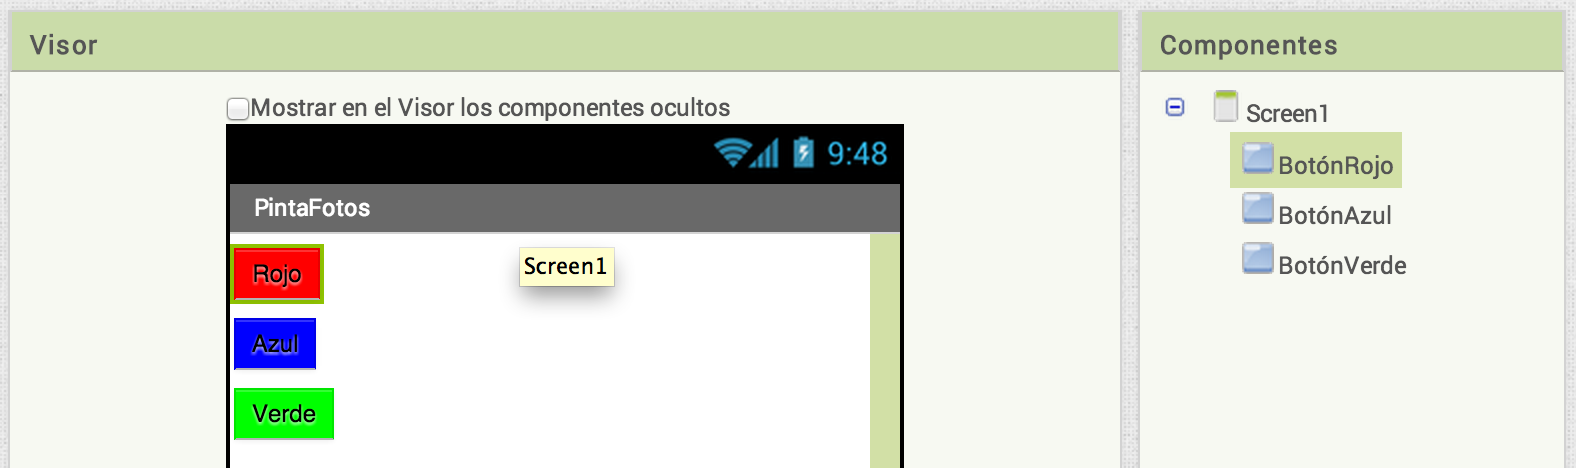
\includegraphics[scale=0.3]{PaintPot1}
\caption{El \viewer con los tres botones creados.}
\label{fig:PaintPot1}
\end{figure}

\paragraph{Importante!}
Observa que en este proyecto cambias los nombres de los componentes en
vez de dejarlos con sus nombres por defecto, como lo hiciste en
\appName{Hola Gatito}. El usar nombres más significativos hace que tus
proyectos sean más fáciles de leer, y realmente ayuda en el momento de
pasar al \blockEditor cuando tendrás que referirte a los componentes
por su nombre. A partir de ahora y en el resto del taller usaremos la
convención de que cada nombre de componente empiece por su tipo (por
ejemplo: \component{BotónRojo}).

\paragraph{Prueba tu aplicación!} Conecta tu aplicación a tu
dispositivo y verifica que funcione correctamente.

\subsubsection*{Usando los Componentes de Disposición para una Mejor
  Presentación}

Ahora deberías tener tres botones alineados verticalmente. Sin embargo
para esta app, vas a necesitar que estén en fila horizontal arriba de
la pantalla, como en la~\Cref{fig:PaintPot2}. Para ello debes usar el
componente \component{DisposiciónHorizontal}.

\begin{figure}[H]
\centering
% 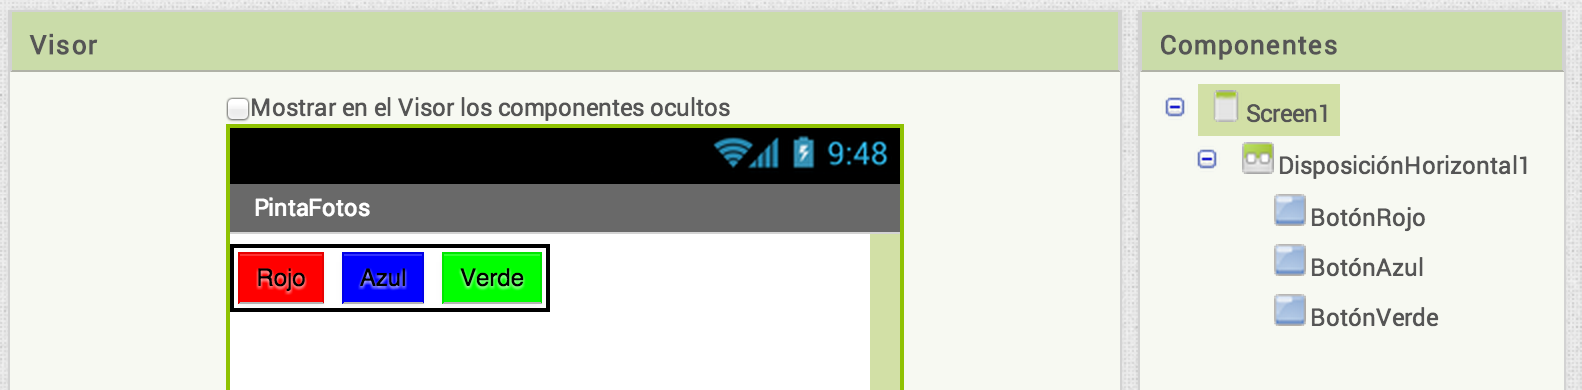
\includegraphics[scale=0.3]{PaintPot2}
\caption{Los tres botones en disposición horizontal.}
\label{fig:PaintPot2}
\end{figure}

\begin{enumerate}

\item Desde la categoría “Disposición'' en la \palette, arrastra un
  componente \component{DisposiciónHorizontal} y ponlo debajo de los
  botones.

\item En el panel de \properties, cambia el \property{Ancho} de
  \component{DisposiciónHorizontal} a la opción ``Ajustar al
  contenedor'' para llenar todo lo ancho de la pantalla.

\item Mueve los tres botones uno después del otro al interior de la
  \component{DisposiciónHorizontal}. \emph{Truco}: Verás una línea
  vertical azul que indica dónde irá el elemento que estás
  arrastrando.

\end{enumerate}

Si miras en la lista de componentes del proyecto, verás tres botones
listados bajo el componente \component{DisposiciónHorizontal}, lo que
muestra que se trata de sus subcomponentes. Asímismo, observa que
todos los componentes están listados bajo el componente
\component{Screen1}.

\paragraph{Prueba tu Aplicación!} Deberías ver tus tres botones en una
fila horizonal en la pantalla, a pesar de que puedan verse un poco
diferente a como se ven en el \designer. Por ejemplo, el borde de
\component{DisposiciónHorizontal} no aparece en el dispositivo.

En general, se usan los componentes de ``Disposición'' como opciones
de diseño para crear disposiciones simples, verticales, horizontales o
en tablas. También puedes crear disposiciones más complejas insertando
componentes de disposición unos dentro de otros.

\subsubsection*{Agregar el Lienzo}

\begin{itemize}

\item El lienzo es el lugar donde el usuario dibuja círculos y
  líneas. Agregalo, y configura el archivo \mediafile{gatito.png},
  usado en \appName{Hola Gatito}, como su \property{ImagenDeFondo}.

\item Desde la categoría ``Dibujo y Animación'' de la \palette,
  arrastra un \component{Lienzo} hacia el \viewer. Cambia su nombre a
  \component{LienzoDeDibujo}. Configura su \property{Ancho} como
  ``Ajustar al Contenedor'' y su \property{Alto} a 300 pixeles.

\item Recuerda que puedes descargar el archivo \mediafile{gatito.png}
  desde \resources{ProgramaTusIdeas/Dia1/HolaGatito}.

\item Configura la \property{ImagenDeFondo} del
  \component{LienzoDeDibujo} con el archivo \mediafile{gatito.png}. Si
  es necesario, debes subir el archivo.

\item Cambia el \property{ColorDePintura} en el
  \component{LienzoDeDibujo} al color rojo para que cuando
  el usuario inicie la app pero todavía no ha presionado ningun botón,
  sus dibujos sean rojos. Comprueba si lo que has hecho es parecido a
  la~\Cref{fig:PaintPot3}.

\begin{figure}[H]
\centering
% 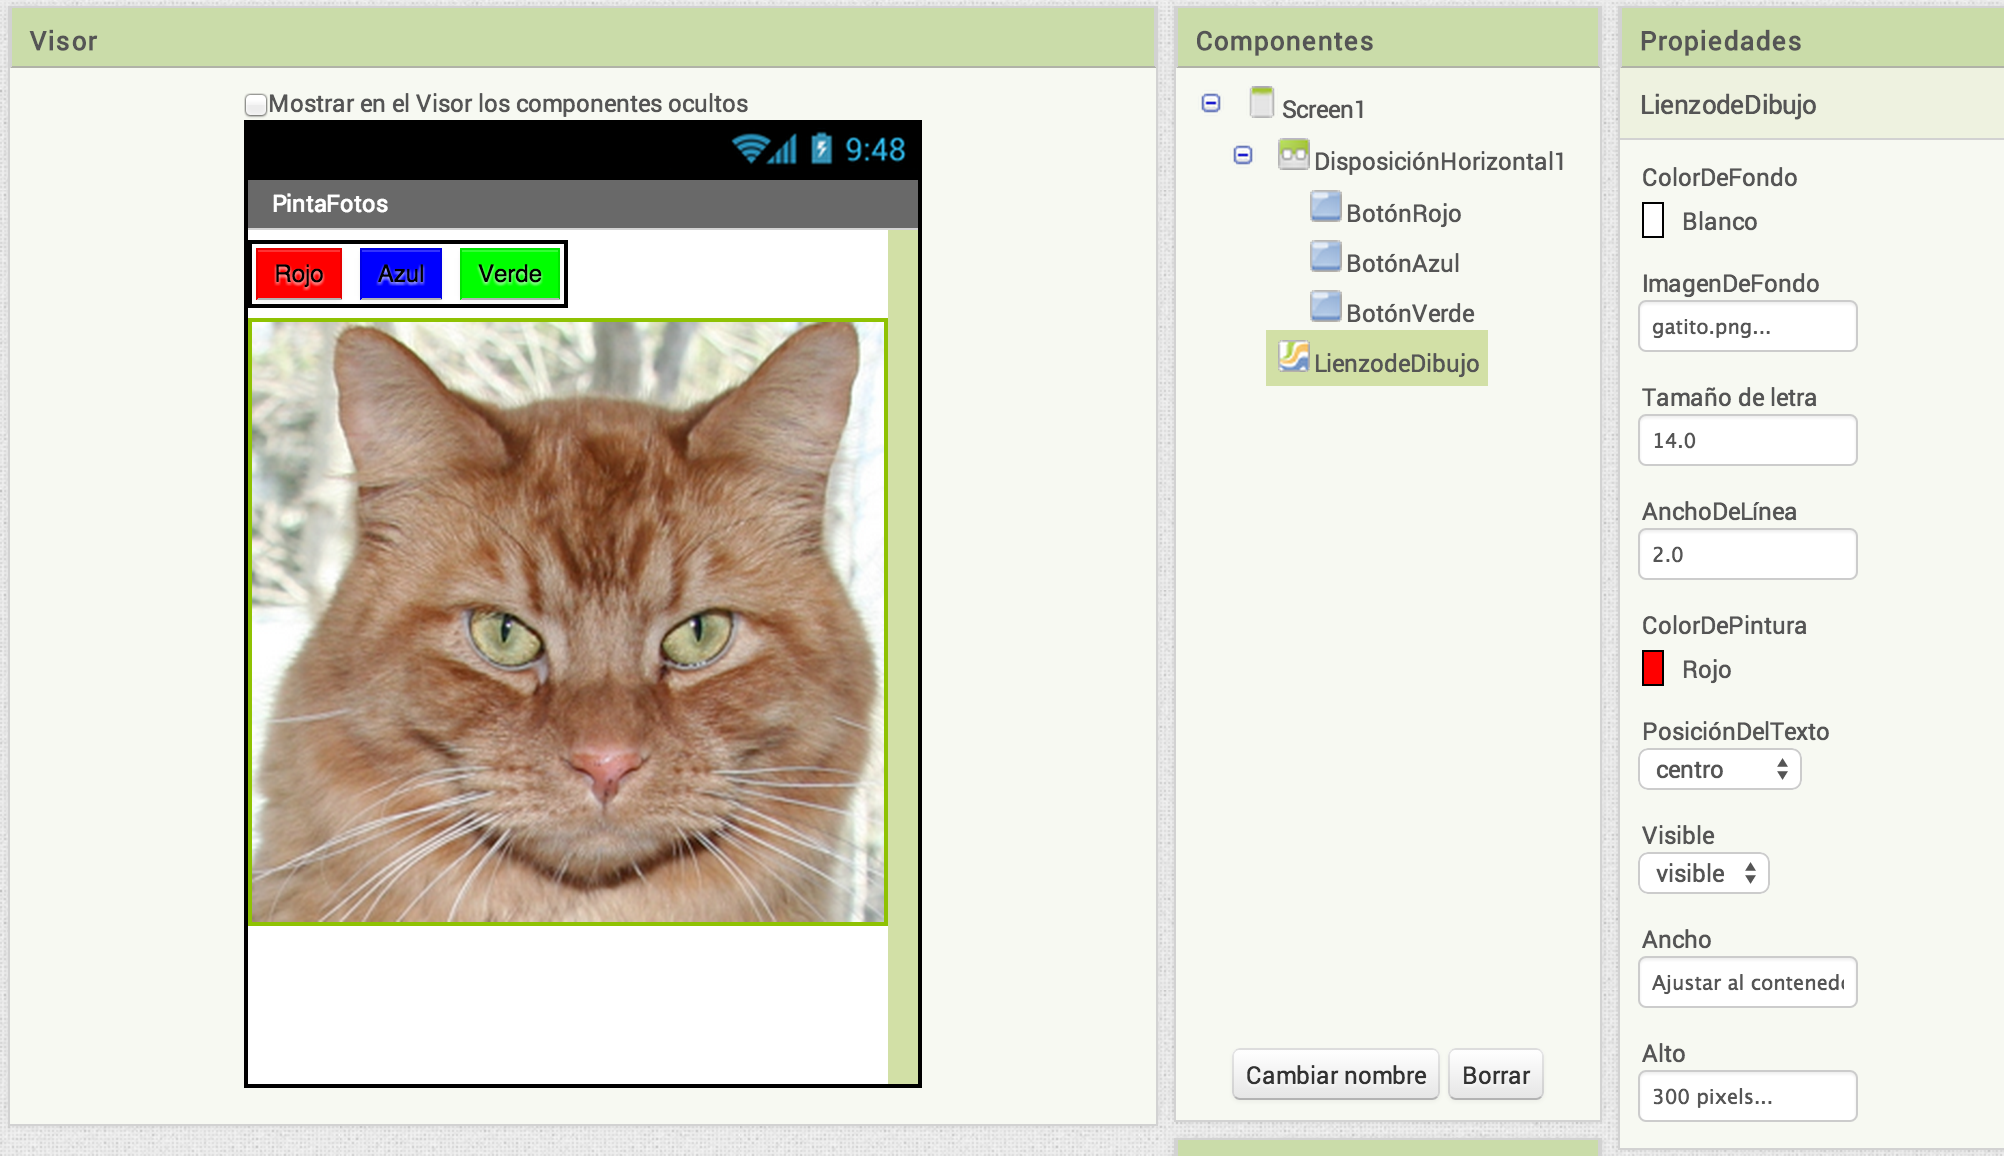
\includegraphics[scale=0.3]{PaintPot3}
\caption{El \component{LienzoDeDibujo} con la imagen
  \mediafile{gatito.png} como \property{ImagenDeFondo}.}
\label{fig:PaintPot3}
\end{figure}

\end{itemize}

\subsubsection*{Agregar los Botones Inferiores y el Componente Cámara}

\begin{enumerate}

\item Desde la \palette, arrastra un nuevo componente
  \component{DisposiciónHorizontal} y ponlo abajo del lienzo.

\item Luego arrastra dos componentes \component{Botón} adicionales en
  el \viewer y ponlos dentro del \component{DisposiciónHorizontal} que
  acabas de agregar. Cambia el nombre del primer botón por
  \component{BotónCámara} y su \property{Texto} a ``Sacar
  Foto''. Cambia el nombre del segundo botón por
  \component{BotónLimpiar} y su \property{Texto} por ``Limpiar''.

\item Arrastra dos botones más y colócalos al lado derecho del
  \component{BotónLimpiar}.

\item Nombra los nuevos botones como \component{BotónGrande} y
  \component{BotónPequeño}, y pon su \property{Texto} como
  ``PuntosGrandes'' y ``PuntosPequeños'' respectivamente.

\item Desde la sección \media de la \palette, arrastra un componente
  \component{Cámara} hacia el \viewer. Aparecerá en la sección de los
  componentes no-visibles.

\end{enumerate}
	
Una vez completados estos pasos, tu aplicación debería verse como en
la~\Cref{fig:PaintPot4}.

\begin{figure}[H]
\centering
% 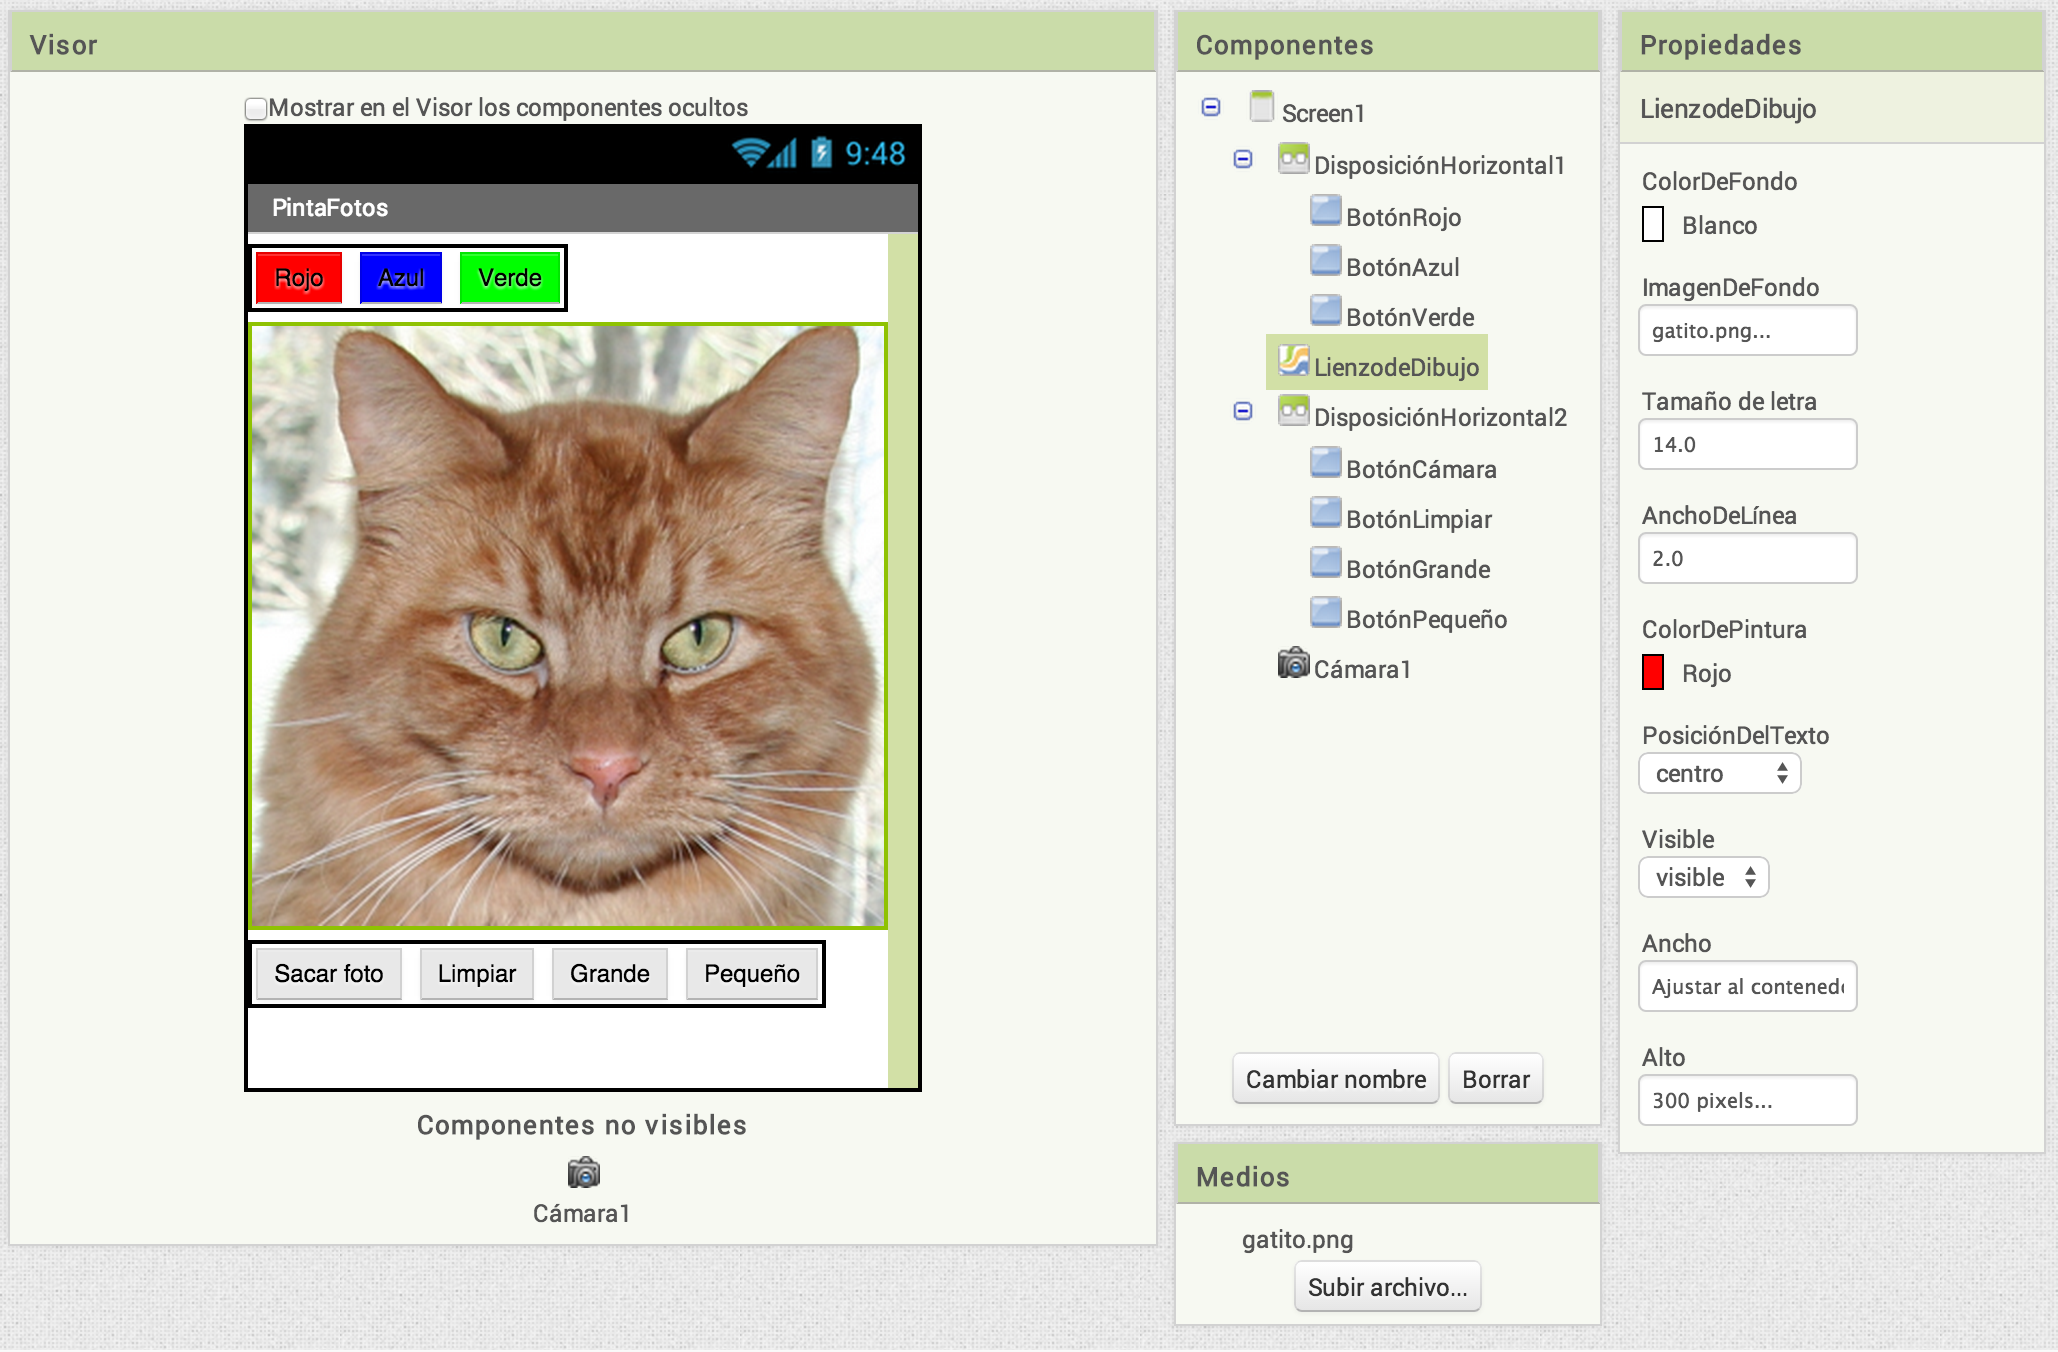
\includegraphics[scale=0.3]{PaintPot4}
\caption{Interfaz de usuario completa para \appName{PintaFotos}}
\label{fig:PaintPot4}
\end{figure}

\paragraph{Prueba tu Aplicación!} ¿Aparece la foto del gatito debajo
de los botones de la primera fila? ¿Aparece la última fila de botones abajo?

\subsubsection*{Agregar Comportamiento a los Componentes}

El próximo paso es definir cómo se comportan los componentes. Crear un
programa de pintura puede parecer un desafío insuperable, pero quedate
tranquilo! \AppInventor te facilita el trabajo: existen bloques muy
fáciles de usar para manejar las funcionalidades de touch y arrastre,
y para dibujar y sacar fotos.

En el \designer, agregaste un componente \component{Lienzo} llamado
\component{LienzoDeDibujo}. Como todos los componentes de ese tipo,
\component{LienzoDeDibujo} tiene un evento \block{Tocar} y un evento
\block{Arrastrado}. Programarás el evento \block{LienzoDibujo.Tocar}
de tal manera que llame a la función
\block{LienzoDibujo.DibujarCírculo}. Programarás el evento
\block{LienzoDibujo.Arrastrado} de tal manera que llame a la función
\block{LienzoDibujo.DibujarLínea}. Programarás luego los botones para
configurar la propiedad \property{ColorDePintura} usando el bloque
\block{poner LienzoDibujo.ColorPintura}, y para limpiar el
\component{LienzoDeDibujo}; y finalmente, programarás como cambiar la
\property{ImagenDeFondo} del lienzo por una foto sacada con la cámara
del dispositivo.

\subsubsection*{Agregar el Evento Tocar para Dibujar un Punto}

Primero, dispondrás los objetos de manera que cuando tocas el
\component{LienzoDeDibujo}, se dibujara un punto en el lugar del lienzo que
toques:
	
\begin{enumerate}

\item En el \blockEditor, selecciona el \component{LienzoDeDibujo}, y
  arrastra el bloque \block{LienzoDeDibujo.Tocado} al \viewer. El
  bloque tiene parámetros para \parameter{x} e \parameter{y},
  y \parameter{spriteTocado}, como ilustrado en
  la~\Cref{fig:PaintPot5}. Estos parámetros entregan información sobre
  la ubicación del evento ``tocar la pantalla'' hecho por el usuario.

\begin{figure}[H]
\centering
% 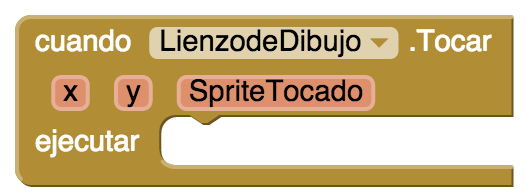
\includegraphics[scale=0.3]{PaintPot5}
\caption{El evento viene con información sobre la ubicación del toque
  en la pantalla}
\label{fig:PaintPot5}
\end{figure}

\textbf{Nota}. Si completaste la aplicación \appName{Hola Gatito}, ya
estás familiarizado con los eventos de \block{Botón.Click}, pero no
con los eventos del lienzo. Los eventos \block{Botón.Click} son
bastante sencillos porque no hay nada más que saber del evento aparte
del hecho que ocurrió. Algunos controladores de eventos, sin embargo,
vienen con información sobre los argumentos para llamar al evento. El
evento \block{LienzoDibujo.Tocar} te entrega las
coordenadas \parameter{x} e \parameter{y} del toque dentro del
\component{LienzoDeDibujo}. También te dice si un objeto dentro del
\component{LienzoDeDibujo} (lo que se conoce como \emph{Sprite}) fue
tocado, pero este punto se abordará más adelante. Las
coordenadas \parameter{x} e \parameter{y} son los argumentos que
usaremos para grabar dónde el usuario tocó la pantalla, de manera de
poder dibujar el punto en este lugar.

\item Arrastra un bloque \block{LienzoDeDibujo.DibujarCírculo} desde
  el bloque y ponlo dentro del controlador de eventos
  \block{LienzoDeDibujo.Tocar}, como se ilustra en
  la~\Cref{fig:PaintPot6}.

\begin{figure}[H]
\centering
% 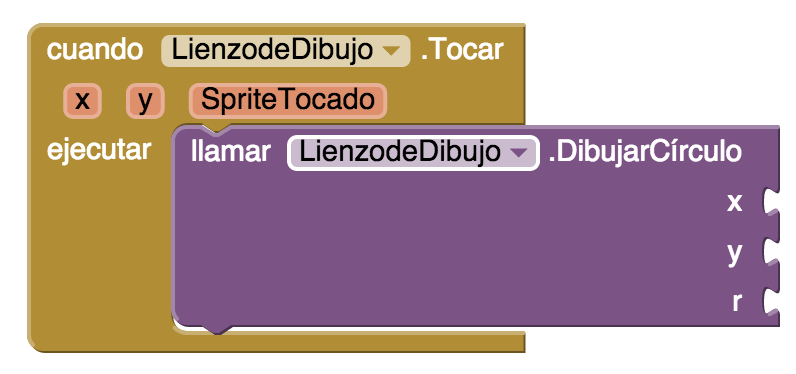
\includegraphics[scale=0.3]{PaintPot6}
\caption{Cuando el usuario toca el lienzo, la aplicación dibuja un círculo}
\label{fig:PaintPot6}
\end{figure}

Por el lado derecho del bloque
\component{LienzoDeDibujo.DibujaCírculo}, verás tres espacios vacíos
por completar con los argumentos
siguientes: \parameter{x}, \parameter{y},
y \parameter{r}. Los \parameter{x} e \parameter{y} especifican la
ubicación donde el círculo se va a dibujar, y \parameter{r} determina
el radio (o tamaño) del círculo.

El signo amarillo con el punto de exclamación a la izquierda inferior
de la pantalla aparecerá con un 1 cuando un espacio todavía permanece
vacío. Construiremos los bloques para completar esto después.

Este controlador de evento puede confundir un poco porque el evento
\block{LienzoDeDibujo.Tocar} también tiene una \parameter{x} y
una \parameter{y}. Solamente acuérdate que la \parameter{x} y
la \parameter{y} para el evento \block{LienzoDeDibujo.Tocar} te dice
dónde tocó el usuario, mientras que el \parameter{x} e \parameter{y}
para el evento \block{LienzoDeDibujo.DibujarCírculo} son espacios
abiertos para que tú definas donde el se dibujará el círculo. Dado que
quieres que el círculo aparezca donde tocó el usuario, conectarás los
valores \parameter{x} e \parameter{y} desde el
\block{LienzoDeDibujo.Tocar} de la misma forma que los valores de los
parámetros \parameter{x} e \parameter{y} en
\block{LienzoDeDibujo.DibujarCírculo}.

Nota. Puedes acceder a los valores del evento al pasar el mouse sobre
los parámetros en el bloque ``Cuando''. Al hacerlo, aparecerán los
bloques \block{tomar} y \block{poner a}. Arrastra el bloque
\block{tomar x} y conéctalo como el valor faltante en
para \parameter{x} en \block{LienzoDeDibujo.DibujarCírculo}, como se
ilustra en la~\Cref{fig:PaintPot7}.

\begin{figure}[H]
\centering
% 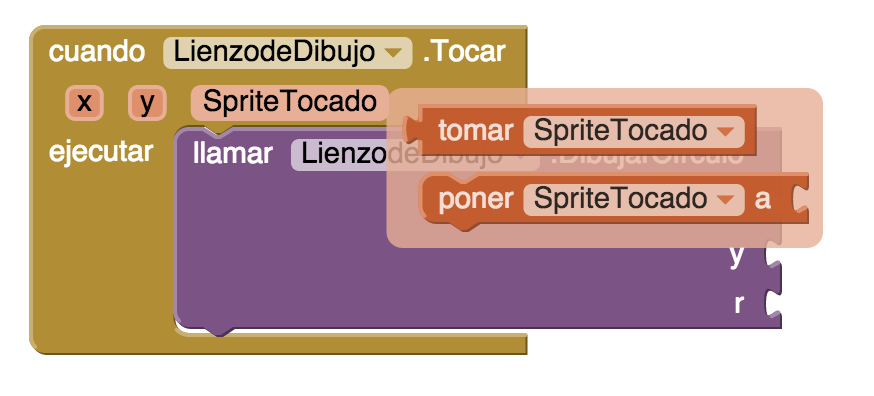
\includegraphics[scale=0.3]{PaintPot7}
\caption{Para acceder al parámetro de un evento, arrastra un bloque
  \block{tomar} desde el bloque \block{LienzoDeDibujo.Tocar}}
\label{fig:PaintPot7}
\end{figure}

\item Arrastra los bloques \block{tomar x} y \block{tomar y} y
  conéctalos en los espacios abiertos en el bloque
  \block{LienzoDeDibujo.DibujarCírculo}, como se ilustra en
  la~\Cref{fig:PaintPot8}.

\begin{figure}[H]
\centering
% 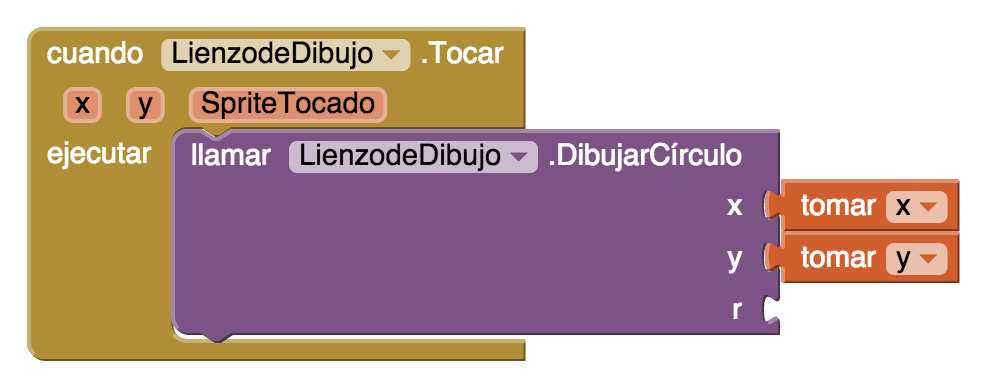
\includegraphics[scale=0.3]{PaintPot8}
\caption{La aplicación sabe donde dibujar (x,y), pero todavía necesitamos
  especificar cuán grande debería ser el círculo.}
\label{fig:PaintPot8}
\end{figure}

\item Ahora necesitas especificar el radio del círculo a dibujar. El
  radio se mide en \emph{pixeles}, que es el punto más pequeño que
  puede ser dibujado en la pantalla. Por ahora, ponle como valor el
  número 5: haz click en una zona blanca de la pantalla y tipea 5,
  luego presiona Enter para crear automáticamente un bloque numérico,
  y conecta este bloque en el espacio para el
  parámetro \parameter{r}. Cuando hagas esto, el signo amarillo en la
  esquina inferior se pondrá en 0 nuevamente, dado que todos los
  espacios abiertos habrán sido completados. La~\Cref{fig:PaintPot9}
  muestra como debiera verse el controlador de eventos
  \block{LienzoDeDibujo.Tocar}.

\begin{figure}[H]
\centering
% 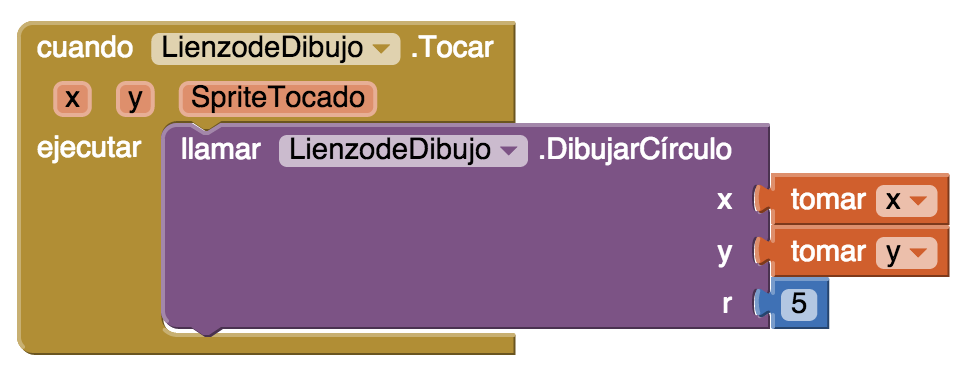
\includegraphics[scale=0.3]{PaintPot9}
\caption{Cuando el usuario toca el \component{LienzoDeDibujo}, un
  círculo de radio 5 será dibujado en las coordenadsa (x, y)
  correspondientes.}
\label{fig:PaintPot9}
\end{figure}

  \textbf{Nota}. Al poner un 5 en el \blockEditor y luego presionar
  Enter, habrás usado lo que se llama \emph{tipeo de bloques}. Si
  empiezas a tipear, el editor de bloques muestra un listado de
  bloques cuyos nombres corresponden a lo que estás tipeando. Si
  tipeas un número, crea un bloque numérico.

  \paragraph{Prueba tu Aplicación!} Usa tu dispositivo para probar lo
  que has desarrollado hasta ahora. Toca el
  \component{LienzoDeDibujo}, tu dedo debería dejar un punto en cada
  lugar que toques. Los puntos serán rojos si configuraste la
  propiedad del \property{LienzoDeDibujo.ColorDePintura} como color
  rojo en el \designer (sino será negro, que es el color por defecto).

\end{enumerate}

\subsubsection*{Agregar el Evento de Arrastre para Dibujar una Línea}

Luego, agregarás el controlador de eventos de arrastre. La diferencia
entre un touch y un arrastre es la siguiente:
	
\begin{itemize}
\item Un touch es cuando pones tu dedo en la pantalla y solo lo
  levantas para tocar, sin desplazarlo.

\item Un arrastre es cuando pones tu dedo en la pantalla y lo mueves
  al mantener contacto con la pantalla.
\end{itemize}
	
En un programa de pintura, cuando arrastras tu dedo en la pantalla se
dibuja una línea igual al camino que sigue tu dedo. Lo que estás
haciendo en realidad es dibujar cientos de pequeñas líneas rectas;
cada vez que mueves tu dedo, incluso un poco, extiendes la línea desde
la última posición de tu dedo hacia su nueva posición.

\begin{enumerate}
	
\item En el \blockEditor, desde la sección del
  \component{LienzoDeDibujo}, arrastra el bloque
  \block{LienzoDeDibujo.Arrastrado} al espacio de trabajo. Deberías
  ver el gestionador de eventos tal como en la~\Cref{fig:PaintPot10}.

\begin{figure}[H]
\centering
% 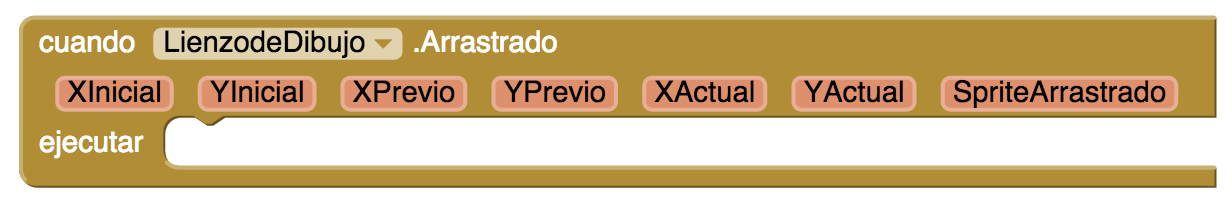
\includegraphics[scale=0.3]{PaintPot10}
\caption{Un evento de arrastre tiene más argumentos que un evento de touch.}
\label{fig:PaintPot10}
\end{figure}

El evento LienzoDibujo.Arrastre viene con los siguientes argumentos:

\begin{itemize}

\item \parameter{XInicial}, \parameter{YInicial}: la posición de tu
  dedo donde empieza el arrastre.

\item \parameter{XActual}, \parameter{YActual}: la posición actual de
  tu dedo.

\item \parameter{XPrevio}, \parameter{YPrevio}: la posición
  inmediatamente anterior de tu dedo.

\item \parameter{SpriteArrastrado}: un booleano, será verdad si el
  usuario hace el arrastre directamente sobre un imagen Sprite. En el
  taller no usaremos este argumento.

\end{itemize}

\item Arrastra el bloque \block{LienzoDeDibujo.DibujarLínea} dentro
  del bloque \block{LienzoDeDibujo.Arrastrado} como se muestra en
  la~\Cref{fig:PaintPot11}.

\begin{figure}[H]
\centering
% 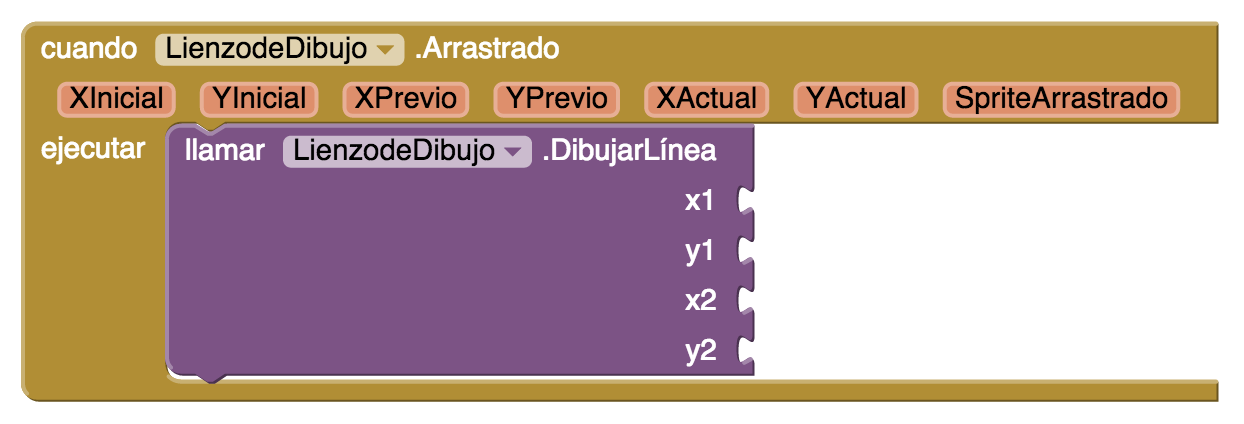
\includegraphics[scale=0.3]{PaintPot11}
\caption{Agregando la habilidad de dibujar líneas}
\label{fig:PaintPot11}
\end{figure}

El bloque \block{LienzoDeDibujo.DibujarLínea} tiene cuatro argumentos,
dos para cada punto que determina la línea: un punto es
(\parameter{x1}, \parameter{y1}), mientras que
(\parameter{x2}, \parameter{y2}) es el otro. ¿Puedes adivinar qué
valores corresponden a cada argumento?  Recuerda que el evento
\block{LienzoDeDibujo.Arrastrado} se activará cada vez que arrastres
tu dedo en el \viewer, por lo tanto la aplicación dibuja una pequeña
línea cada vez que mueves tu dedo, desde
(\parameter{XPrevio}, \parameter{YPrevio}) hacia
(\parameter{XActual}, \parameter{YActual}). Agreguemos esto a nuestro
bloque \block{LienzoDeDibujo.DibujarLínea}:

\item Arrastra los bloques \block{tomar} para los argumentos que vas a
  necesitar. Los valores \parameter{XPrevio} e \parameter{YPrevio}
  deberían ir conectados en los espacios para los
  argumentos \parameter{x1} e \parameter{y1}, respectivamente, como se
  ilustra en la~\Cref{fig:PaintPot12}.

\begin{figure}[H]
\centering
% 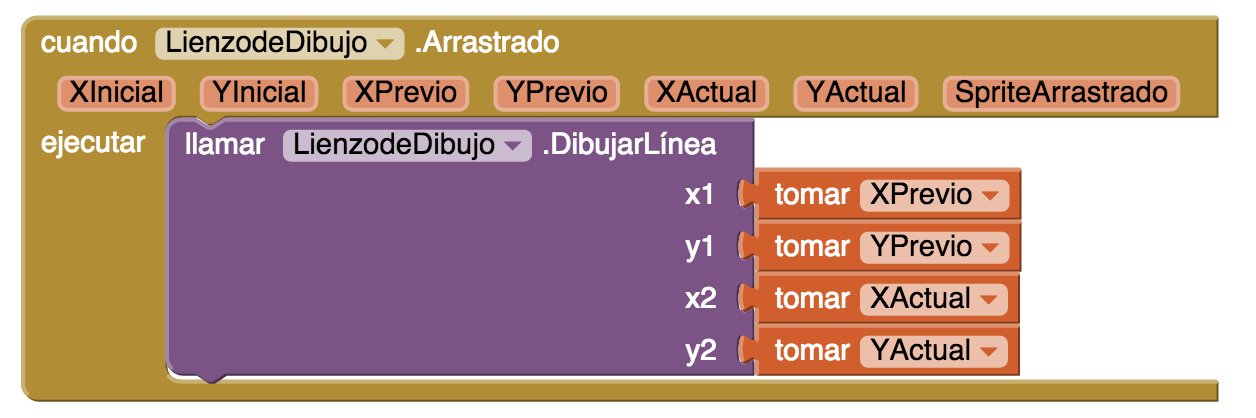
\includegraphics[scale=0.3]{PaintPot12}
\caption{Cuando el usuario arrastre el dedo, la aplicación dibujará
  una línea desde el punto anterior hacia el actual.}
\label{fig:PaintPot12}
\end{figure}

\paragraph{Prueba tu Aplicación!} Arrastra tu dedo en la pantalla para
dibujar líneas y curvas. Toca la pantalla para dibujar puntos.

\end{enumerate}

\subsubsection*{Agregar Controladores de Eventos para Botones}

La aplicación que has construido hasta ahora permite al usuario
dibujar, pero siempre estos dibujos usan el color rojo. El próximo
paso consiste en agregar controladores de eventos para los botones de
colores, para que el usuario pueda cambiar el color de la pintura, y
otro para el \component{BotónLimpiar} para que pueda limpiar la
pantalla y así volver a empezar a dibujar.

En el \blockEditor:

\begin{enumerate}
\item Arrastra el bloque \block{BotónRojo.Click} al espacio de
  trabajo.

\item Arrastra el bloque \block{poner LienzoDeDibujo.ColorDePintura} y
  conéctalo en las acciones del bloque \block{BotónRojo.Click}.

\item Abre la sección ``Colores'' y arrastra el bloque de color rojo
  para conectarlo con el bloque \block{poner
    LienzoDeDibujo.ColorDePintura}.

\item Repite los pasos anteriores para los botones azul y verde.

\item El último botón por configurar es el
  \component{BotónLimpiar}. Para limpiar el lienzo de dibujo debes
  utilizar el bloque \block{LienzoDeDibujo.Limpiar}. Confirma que tus
  bloques se ven como en la~\Cref{fig:PaintPot13}.

\begin{figure}[H]
\centering
% 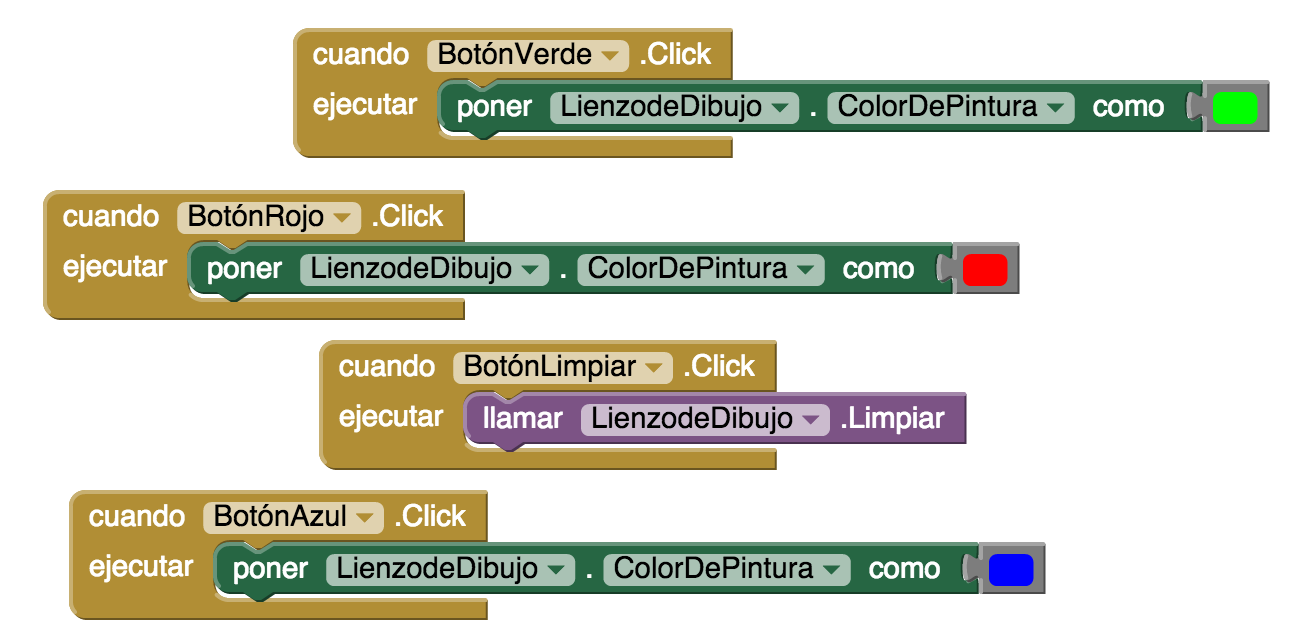
\includegraphics[scale=0.3]{PaintPot13}
\caption{Cuando el usuario hace click en los botones de colores cambia
el color para dibujar en el lienzo. Hacer click en ``Limpiar'', borra
el contenido del lienzo.}
\label{fig:PaintPot13}
\end{figure}

\end{enumerate}

\subsubsection*{Permitir al Usuario Tomar un Foto}

Las aplicaciones hechas con \AppInventor pueden interactuar con las
funcionalidades de los dispositivos Android, incluyendo la
cámara. Para personalizar la aplicación, se permite al usuario fijar
la imagen de fondo de su dibujo con una foto tomada con la cámara.

\begin{enumerate}

\item El componente \component{Cámara} contiene dos bloques claves. El
  bloque \block{Cámara.TomarFoto} inicia la aplicación de cámara del
  teléfono. El evento \block{Cámara.DespuésDeTomarFoto} se activa
  cuando el usuario terminó de sacar la foto. Agregarás bloques en el
  controlador de eventos \block{Cámara.DespuésDeTomarFoto} para
  configurar el \block{LienzoDeDibujo.ImagenDeFondo} con la foto que
  fue sacada. Abre la sección de \component{BotónCámara} y arrastra el
  controlador de evento \component{BotónCámara.Click} hacia el espacio
  de trabajo.

\item Arrastra el bloque \block{Cámara1.TomarFoto} y ponlo en el
  controlador \block{BotónCámara.TomarFoto}.

\item Arrastra el controlador de eventos
  \block{Cámara1.DespuésDeTomarFoto} al espacio de trabajo.

\item Arrastra el bloque \block{poner LienzoDeDibujo.ImagenDeFondo} y
  ponlo en las acciones de \block{Cámara1.DespuésDeTomarFoto}.

\item \block{Cámara1.DespuésDeTomarFoto} tiene un argumento
  llamado \parameter{imagen}, que es la foto recién sacada. Puedes
  referirte a ella, con un bloque ``tomar'' desde el bloque
  \block{Cámara1.DespuésDeTomarFoto}. Conecta la imágen como el
  argumento para el bloque \block{poner LienzoDeDibujo.ImagenDeFondo}.
	
  Los bloques deberían ser parecidos a la~\Cref{fig:PaintPot14}.

\begin{figure}[H]
\centering
% 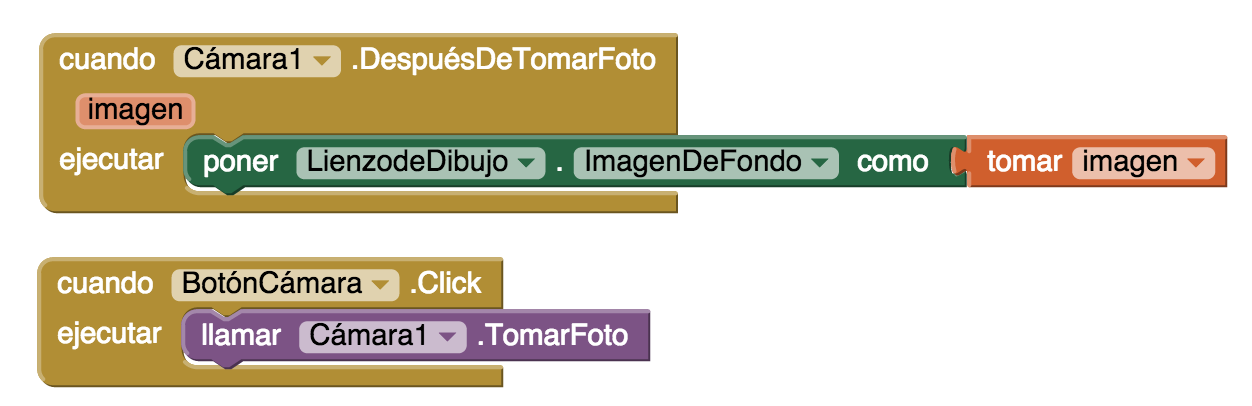
\includegraphics[scale=0.3]{PaintPot14}
\caption{CUando se saca la foto, se configura como la imagen de fondo
  del lienzo.}
\label{fig:PaintPot14}
\end{figure}

\paragraph{Prueba tu Aplicación!} Haz una prueba al hacer click en
``Tomar Foto'' y saca una foto. El gatito debería cambiar por la foto
que acabas de sacar, y luego podrás dibujar encima de la foto que
sacaste.

\end{enumerate}

\subsubsection*{Cambiar el Tamaño del Punto}

El tamaño de los puntos dibujados en el \component{LienzoDeDibujo} se
determina al llamar a \block{LienzoDeDibujo.DibujarCírculo}, donde el
argumento de radio está configurado en 5. Para cambiar el grueso de la
línea, puedes cambiar el valor de \parameter{r}. Para probar esto,
intenta cambiar el 5 por un 10 y pruébalo en el teléfono para ver cómo
aparece.

El único tamaño que el usuario podrá usar es él que tu indicas como
argumento para el radio del círculo. ¿Pero qué pasa si el usuario
quiere cambiar el tamaño de los puntos? Vamos a modificar el programa
de manera que el usuario---no solo el programador---pueda cambiar el
tamaño de los puntos. Lo haremos de tal manera que cuando el usuario
haga click en un botón llamado ``Grandes'', el tamaño será 8, y cuando
hará click en un botón llamado ``Pequeños'', será 2.

Para usar distintos valores en el argumento radio, la aplicación
necesita saber cuál queremos aplicar. Necesitamos pedirle usar un
valor específico, y tiene que memorizar este valor de manera a poder
seguir usándolo. Cuando tu aplicación necesita guardar algo en memoria
que no sea una propiedad, puedes definir una \emph{variable}. Una
variable es una \emph{celda de memoria}. Es como un balde donde puedes
almacenar datos variables, como el tamaño del punto.

Empezamos por definir una variable \variable{TamañoPunto}:

\begin{enumerate}

\item En el \blockEditor, desde la sección ``Variables'', arrastra un
  bloque \block{Inicializar global nombre}. Cambia el texto
  ``nombre'' por ``TamañoPunto''.

\item Fíjate que el bloque \block{Inicializar global TamañoPunto}
  tiene un espacio abierto. Ahí es donde puede especificar el valor
  inicial de la variable, o su valor por defecto al iniciar la
  aplicación. Para esta aplicación, inicializa el
  \variable{TamañoPunto} en 2 creando un bloque con el número 2, y
  conectándolo en \block{Inicializar global TamañoPunto} como se
  ilustra en la~\Cref{fig:PaintPot15}.
\end{enumerate}

\begin{figure}[H]
\centering
% 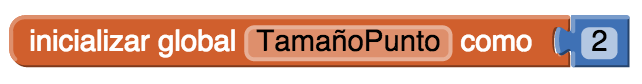
\includegraphics[scale=0.3]{PaintPot15}
\caption{Inicializar variable global \variable{TamañoPunto} con valor
  2.}
\label{fig:PaintPot15}
\end{figure}

\subsubsection*{Usar las Variables}

Ahora, queremos cambiar el argumento de
\block{LienzoDeDibujo.DibujarCírculo} en el controlador de eventos
\block{LienzoDibujo.Tocar} para que uses el valor
\variable{TamañoPunto} en vez de usar siempre un número fijo. (Puede
dar la ilusión que fijamos \variable{TamañoPunto} en 2 porque lo
inicializamos de esta manera, pero verás en un minuto como podemos
cambiar \variable{TamañoPunto} y asi cambiar el tamaño del punto que
se dibuja.)

\begin{enumerate}
\item Arrastra un bloque ``tomar'' desde
  \block{LienzoDeDibujo.DibujarCírculo}. Deberías ver un bloque
  \block{tomar global TamañoPunto} que indica el valor de la variable.

\item Anda al controlador de eventos \block{LienzoDeDibujo.Tocar} y
  arrastra el bloque del número 5 fuera del espacio \parameter{r} y
  pónlo en el papelero.  Luego reemplázalo con el bloque \block{tomar
    global TamañoPunto} (Ver~\Cref{fig:PaintPot16}). Cuando el usuario
  toca el lienzo, la aplicación determinará ahora el radio a partir de
  la variable \variable{TamañoPunto}.
\end{enumerate}

\begin{figure}[H]
\centering
% 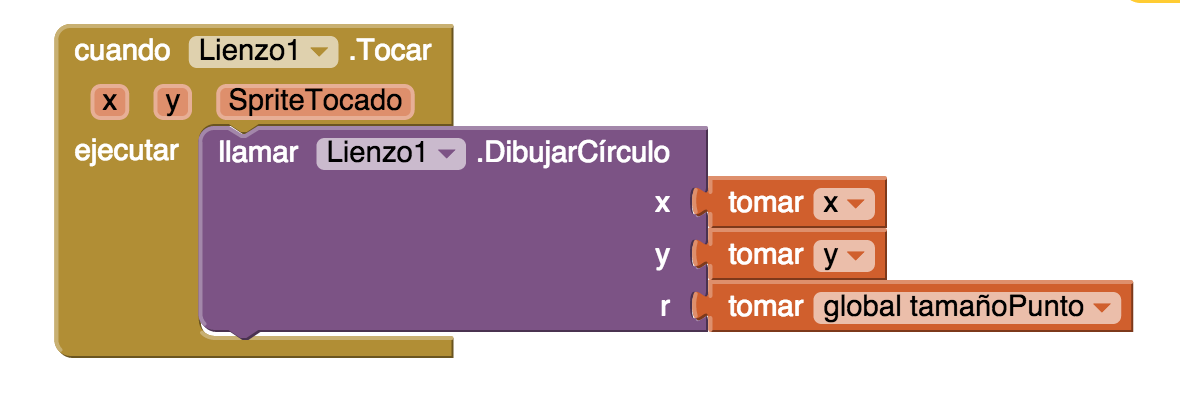
\includegraphics[scale=0.3]{PaintPot16}
\caption{Ahora el tamaño de cada círculo depende de lo
que está guardado en la memoria de la variable TamañoPunto.}
\label{fig:PaintPot16}
\end{figure}

\subsubsection*{Cambiar los valores de las variables}

Aquí es donde la magia de las variables opera. La variable
\variable{TamañoPunto} permite al usuario elegir el tamaño del
círculo, y tu controlador de eventos dibujará el círculo en función de
esto.  Desarrollaremos el comportamiento al programar los
controladores de eventos \block{BotónPequeño.Click} y
\block{BotónGrande.Click}.

\begin{enumerate}

\item Arrastra un controlador de eventos \block{BotónPequeño.Click}
    al espacio de trabajo. Luego arrastra desde la categoría
    ``Variables'' un bloque \block{poner a}, selecciona ``global
    TamañoPunto'' como referencia y conectalo a
    \block{BotónPequeño.Click}. Finalmente, crea un bloque número 2 y
    conéctalo al bloque \block{poner global TamañoPunto}.

\item Haz un controlador de eventos similar para
  \block{BotónGrande.Click}, pero configura el \variable{TamañoPunto} en 8. Ambos gestionadores de eventos
  deberían aparecer en el editor de bloques, como en la~\Cref{fig:PaintPot17}.

\end{enumerate}

\begin{figure}[H]
\centering
% 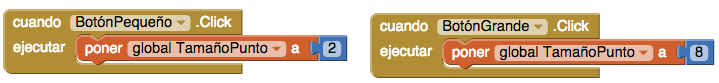
\includegraphics[scale=0.3]{PaintPot17}
\caption{Hacer click en los botones cambia el tamaño del
punto. Los toques que siguen serán con este tamaño de punto.}
\label{fig:PaintPot17}
\end{figure}

\paragraph{Prueba tu Aplicación!} Intenta hacer click en los botones
de tamaño y luego toca el lienzo. ¿Se dibujan círculos de distintos
tamaños? ¿Las líneas? El tamaño de las líneas no debería cambiar
porque programaste \variable{TamañoPunto} solamente para ser usado en
el bloque de \block{DibujarCírculo}. En base a esto, ¿podrías ahora
cambiar tus bloques para que el usuario también pueda cambiar el
tamaño de la línea? (Nota que el lienzo tiene una propiedad llamada
\property{AnchodeLinea})

\subsubsection*{La App Completa: PintaFotos}

La~\Cref{fig:PaintPot18} ilustra el código completo de la aplicación \appName{PintaFotos}:

\begin{figure}[H]
\centering
% 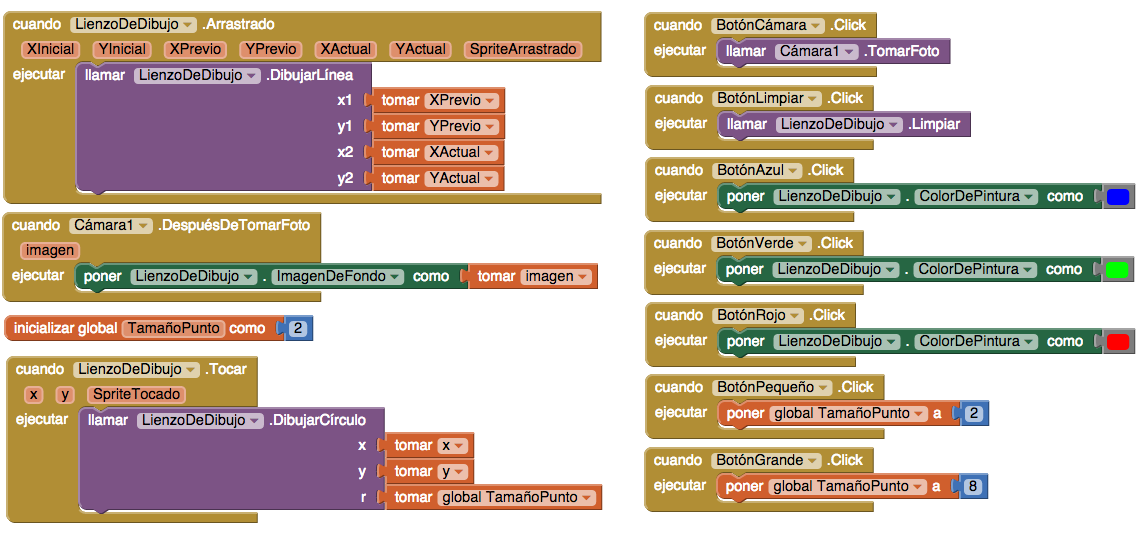
\includegraphics[scale=0.3]{PaintPot18}
\caption{Grupos de bloques para \appName{PintaFotos}.}
\label{fig:PaintPot18}
\end{figure}

\subsubsection*{Resumen}

Las ideas claves que hemos visto en este tutorial son las siguientes:

\begin{itemize}

\item El componente \component{Lienzo} te permite dibujar en un
  lienzo. También es sensible a eventos ``touch'' y de arrastre, los
  cuales puedes aprovechar para desarrollar funcionalidades para
  dibujar.

\item Puedes usar componentes de disposición en la pantalla para
  organizar tus componentes en lugar de ponerlos todos uno debajo del
  otro.

\item Algunos controladores de eventos vienen con información sobre el
  evento, como las coordenadas de donde la pantalla fue tocada. Esta
  información está representada por argumentos. Cuando arrastras un
  controlador de eventos que tiene argumentos, \AppInventor crea ítems
  ``poner a'' y ``tomar'', dentro del bloque seleccionado, para así
  poder referirse a estos argumentos.

\item Crear variables al usar bloques \block{poner global nombre},
  desde la categoría ``Variables''. Las variables permiten guardar
  información en memoria, como el tamaño del punto, que no está
  guardado en una propiedad de un componente.

\item Para cada variable que definas, \AppInventor automáticamente
  provee una referencia ``tomar global'' que entrega el valor de la
  variable, y una referencia ``poner global a'' para cambiar el valor
  de la variable. Para acceder a esto, arrastra un bloque ``poner a''
  o ``tomar'' desde el mismo bloque donde declaras la variable.
\end{itemize}

El componente Lienzo también se puede usar para programar animaciones
como las que ves en juegos en 2D.

\section{Discusión y Ejercicios de Personalización}

\begin{enumerate}

\item En el \component{Lienzo}, los controladores de eventos \block{Tocar} y
\block{Arrastrado}, mostrados abajo en la~\Cref{fig:PaintPot20},
tienen parámetros de evento. Nombra cada parámetro e indica lo que
representa.

\begin{figure}[H]
\centering
% 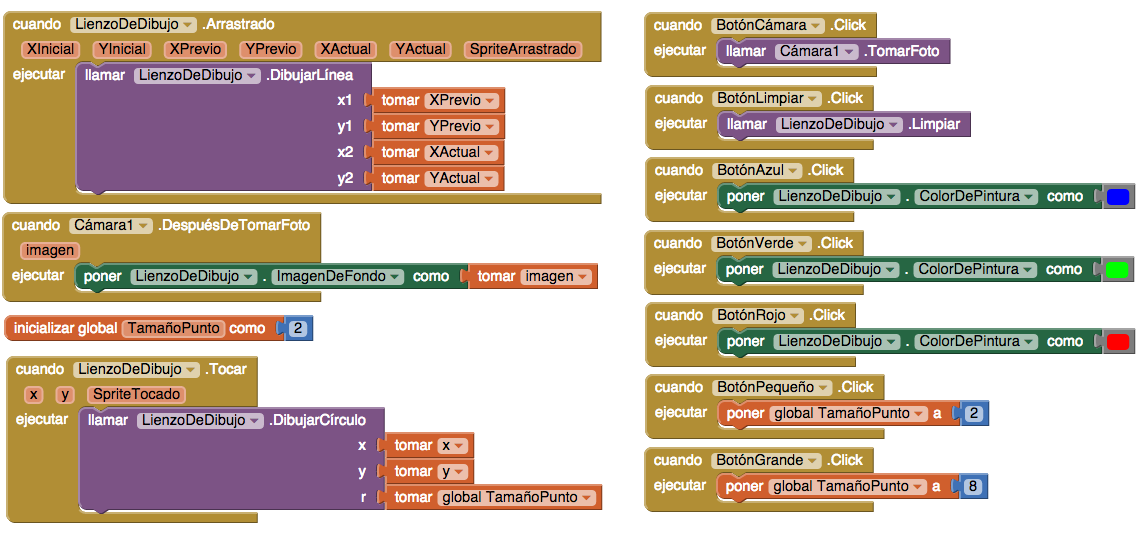
\includegraphics[scale=0.3]{PaintPot18}
\caption{Grupos de bloques para \appName{PintaFotos}.}
\label{fig:PaintPot18}
\end{figure}

\item Los parámetros de evento son distintos de los parámetros para llamar
funciones. ¿Cómo se llaman los parámetros para llamar funciones en el
controlador de eventos de la~\Cref{fig:PaintPot20}? ¿Quién especifica
los parámetros de función? Quién especifica parámetros de eventos?

\item ¿Cuál es el propósito de definir una variable para el Tamaño de Punto
en la App Pinta Fotos? Si quieres permitir cambiar el grosor de las
líneas, ¿necesitarás una variable?

\item Define lo que es una variable. ¿Cuáles son sus puntos en común con una
propiedad? ¿Cómo se diferencia de una propiedad?

\item Una forma de personalizar la aplicación es poner un
  \component{CuadroDeTexto} para el tamaño del punto. ¿Cuál es la
  diferencia entre un cuadro de texto y una variable? ¿Cuál es la
  diferencia entre una etiqueta y un cuadro de texto?

\end{enumerate}

\paragraph{Ejercicios para personalizar la app}

\begin{enumerate}

\item
  La interfaz de usuario de \appName{PintaFoto} no permite mostrar con qué color
  se está dibujando. El usuario sólo se da cuenta al dibujar. ¿Puedes
  agregar esta información para el usuario de tal manera que cuando él
  hace click para cambiar el color, la interfaz cambia y le indica qué
  color fue elegido?

\item
  El tamaño del punto para dibujar un círculo sólo puede ser de 2 o 8.
  ¿Puedes cambiar esto para permitir al usuario elegir entre distintas
  opciones con un componente \component{Deslizador} o un
  \component{CampoDeTexto}?

\item Permitir al usuario controlar el grosor de las líneas, de la
  misma manera que puede cambiar el tamaño del punto. El lienzo tiene
  una propiedad \property{AnchoDeLinea} que controla esta
  característica.
\end{enumerate}

\section{Tutorial: Atrapa el Topo}

\section{Proyecto}

\section{Material de Apoyo}

\subsection*{Componente Lienzo}

\subsection*{Variables}

\subsection*{Temporizadores}


\end{document}
